\documentclass[12pt]{article}
\usepackage[utf8]{inputenc}
\usepackage{graphicx}
\usepackage{courier}
\usepackage[brazilian]{babel}
\usepackage{float}
\usepackage[margin=1in]{geometry}
\usepackage{subfig}

\author{Sofia Catharina Disegna - 16/0018226}
\date{}
\title{Lista 01}
\begin{document}
\tiny
Universidade de Brasília

Faculdade de Tecnologia

Departamento de Engenharia Elétrica

Criptografia Baseada em Caos - 1/2019

\normalsize

{\let\newpage\relax\maketitle}
\section{Exercício 01}
    O objetivo desse primeiro exercício é a simulação do sistema caracterizado pelas seguintes equações:
    \begin{equation}
        \left\{
            \begin{array}{l}
              \dot{x} = z + (y - a)x + u\\
              \dot{y} = 1 - by - x^2\\
              \dot{z} = -x - cz\\
              \dot{u} = -dxy - ku
            \end{array}
          \right.
    \end{equation}

    Esse sistema possui os seguintes parâmetros e condições iniciais:
    \begin{table}[H]%
        \centering
        \subfloat[][]{
            \begin{tabular}{|l|l|}
                \hline
                \multicolumn{2}{|l|}{\textbf{Condições iniciais}} \\ \hline
                x(0)                     & 1                      \\ \hline
                y(0)                     & 2                      \\ \hline
                z(0)                     & 0.5                    \\ \hline
                u(0)                     & 0.5                    \\ \hline
            \end{tabular}
        }%
        \qquad
        \subfloat[][]{
            \begin{tabular}{|l|l|}
                \hline
                \multicolumn{2}{|l|}{\textbf{Constantes}} \\ \hline
                a                     & 0.9                      \\ \hline
                b                     & 0.2                      \\ \hline
                c                     & 1.5                    \\ \hline
                d                     & 0.2                    \\ \hline
                k                     & 0.17                    \\ \hline
            \end{tabular}
            
        }
        \caption{Condições iniciais e constantes do sistema}%
        \label{tbl:table}%
      \end{table}
    \subsection{Simulação do sistema}
    A primeira parte do exercício pede que esse sistema seja simulado em uma janela de tempo, a qual foi escolhida como 20s, e que os gráficos que mostram a evolução no tempo dos parâmetros sejam mostrados.

    Essa simulação foi feita com passo de 1ms entre as iterações e está no script \\
    \texttt{nonlinear\_system\_simulation.m}. Os gráficos obtidos são mostrados abaixo:
    \begin{figure}[H]
        \subfloat[][Variável X]{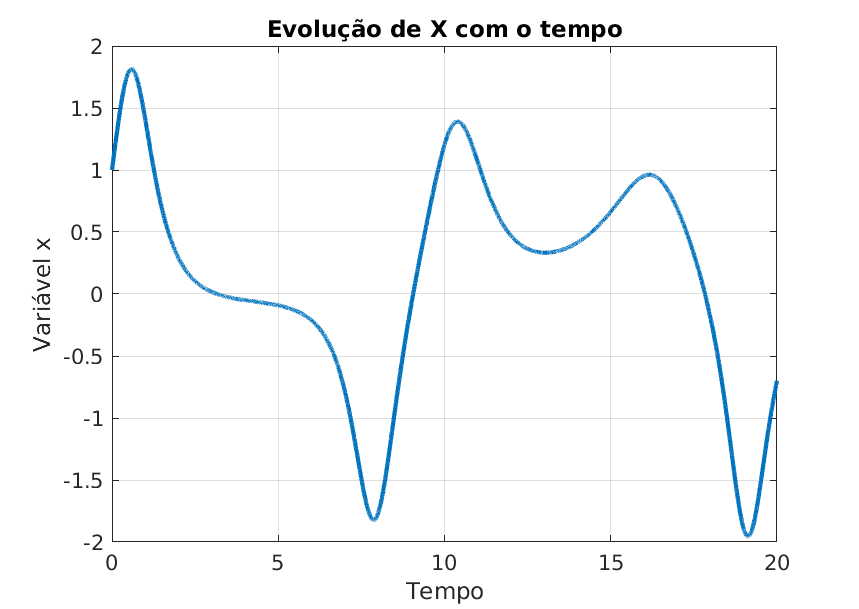
\includegraphics[scale=0.5]{plotx.png}\label{origx}} \qquad
        \subfloat[][Variável Y]{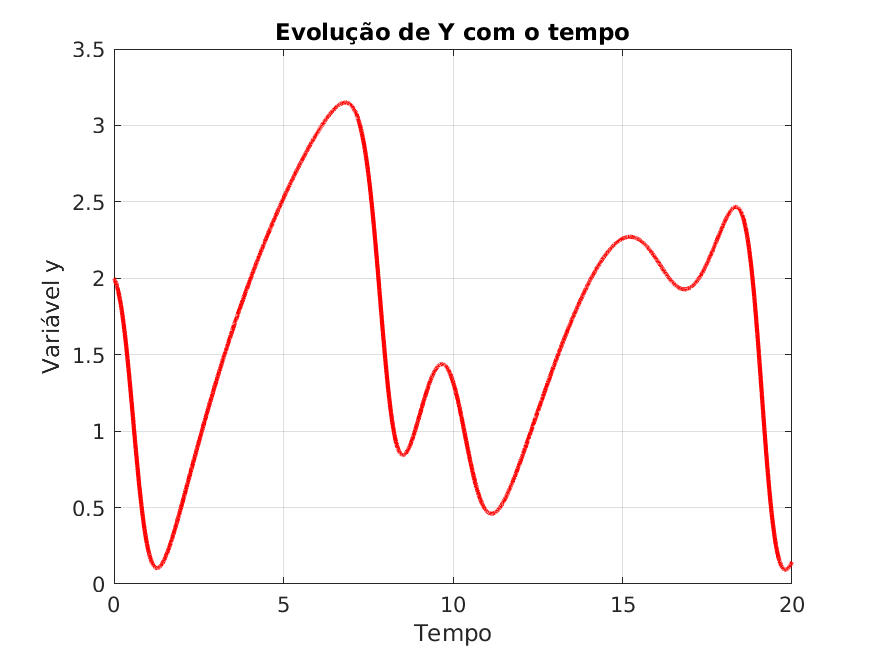
\includegraphics[scale=0.5]{ploty.png}\label{origy}} \par       
        \subfloat[][Variável Z]{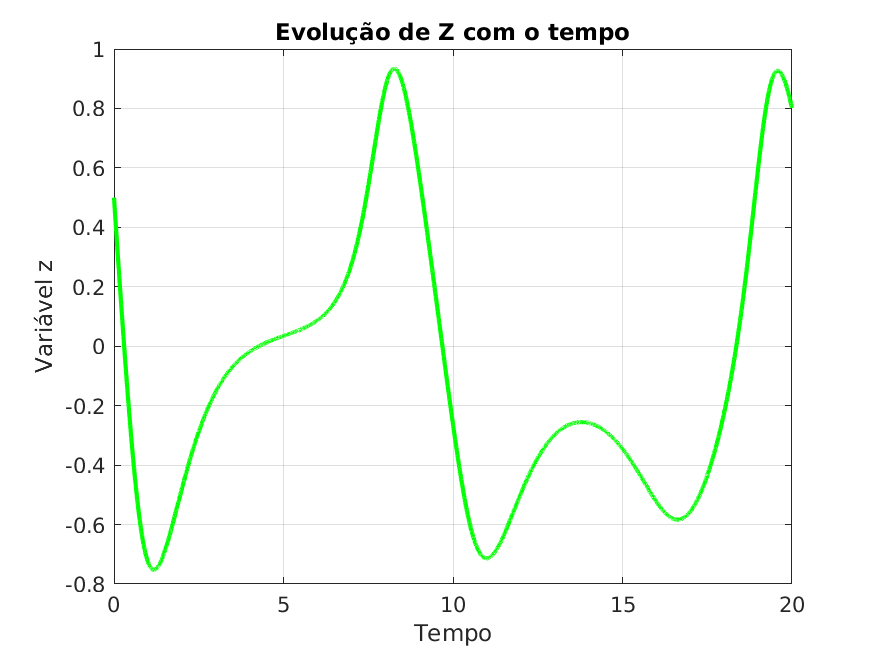
\includegraphics[scale=0.5]{plotz.png}\label{origz}} \qquad
        \subfloat[][Variável U]{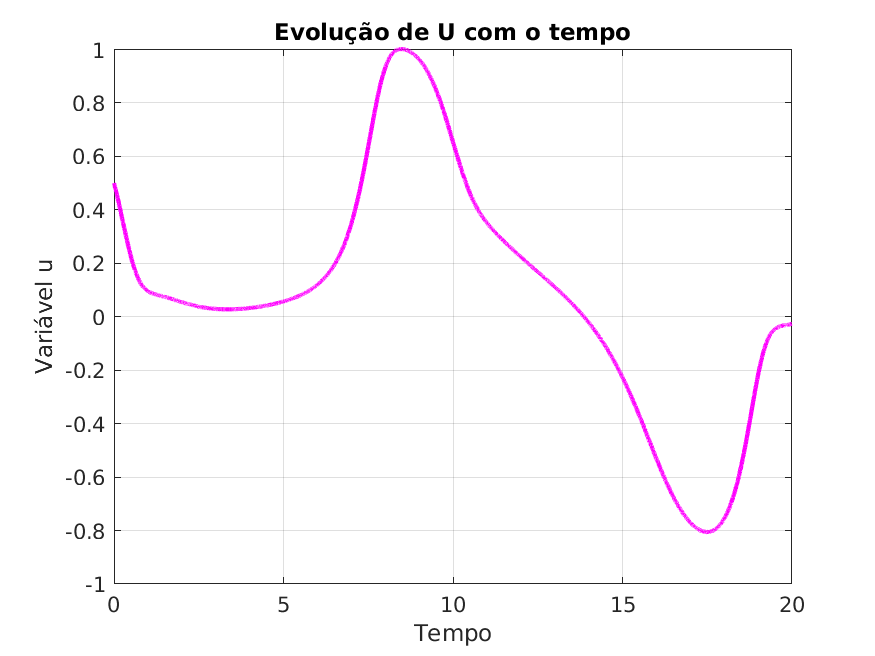
\includegraphics[scale=0.5]{plotu.png}\label{origu}} \par
        \caption{Gráficos das variáveis de estado do sistema no tempo}        
    \end{figure}

    \subsection{Escalonamento no tempo}
    O escalonamento no tempo do sistema pode ser feito com a multiplicação do lado direito pelo fator de escalonamento, sem alterar as constantes e condições iniciais. Nesse caso, o objetivo é acelerar 10 vezes a simulação do sistema, conforme a equação abaixo:
    
    \begin{equation}
        \left\{
            \begin{array}{l}
              \dot{x} = (z + (y - a)x + u)\times 10\\
              \dot{y} = (1 - by - x^2)\times 10\\
              \dot{z} = (-x - cz)\times 10\\
              \dot{u} = (-dxy - ku)\times 10
            \end{array}
          \right.
    \end{equation}

    Nas figuras abaixo, que foram geradas com o script \texttt{time\_scaling.m} podemos ver uma comparação entre os sinais originais e os escalonados no tempo, que mostram que os 20 primeiros segundos do sistema original são iguais aos 2 primieiros segundos do sistema escalonado no tempo:
    \begin{figure}[H]
        \subfloat[][Gráfico do sistema original]{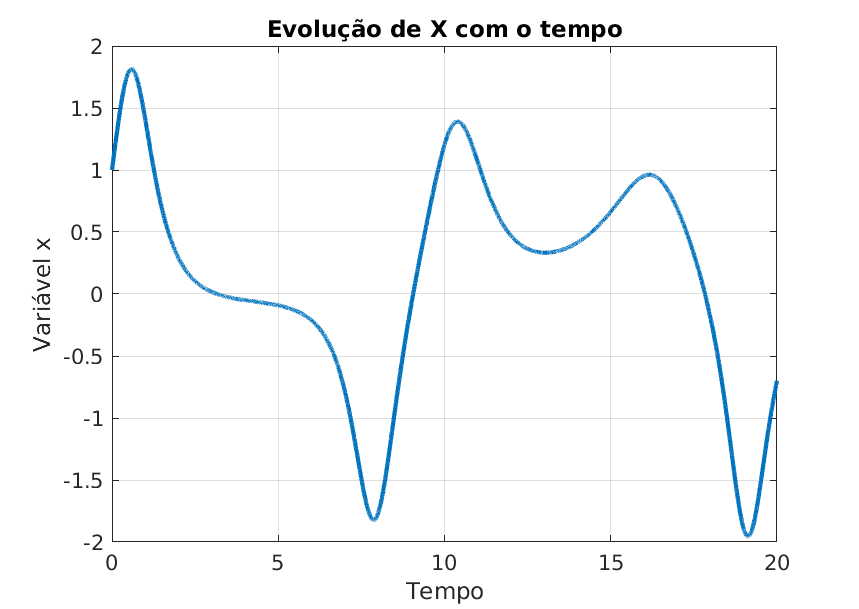
\includegraphics[scale = 0.55]{plotx.png}\label{xorig}}
        \subfloat[][Gráfico do sistema escalonado no tempo]{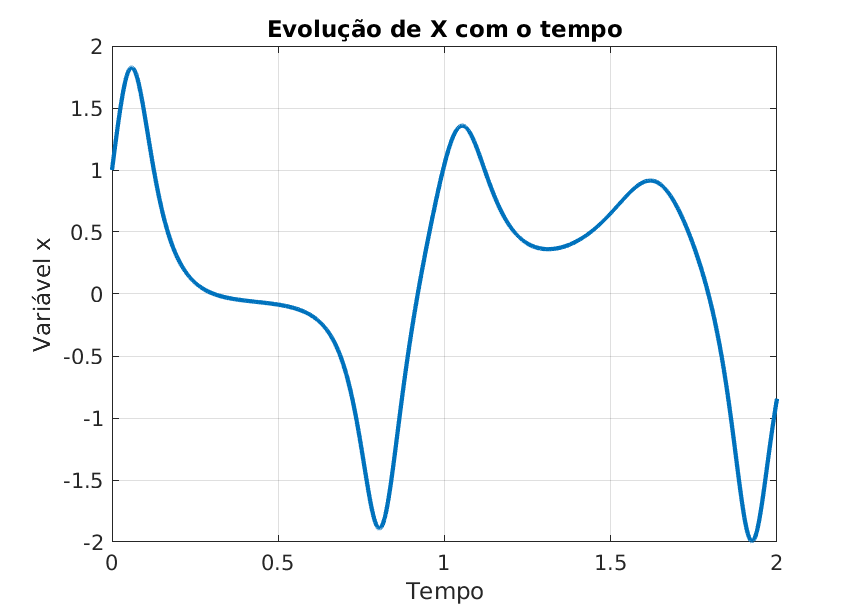
\includegraphics[scale = 0.55]{plotx_timescaled.png}\label{xts}}
        \caption{Comparação entre o sistema original e o escalonado para a variável X}
    \end{figure}

    \begin{figure}[H]
        \subfloat[][Gráfico do sistema original]{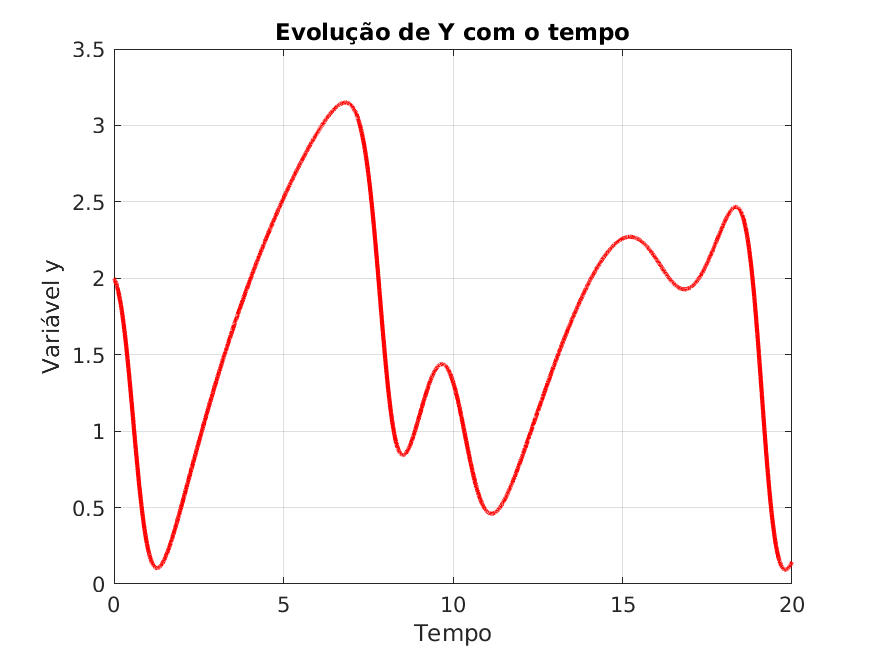
\includegraphics[scale = 0.55]{ploty.png}\label{yorig}}
        \subfloat[][Gráfico do sistema escalonado no tempo]{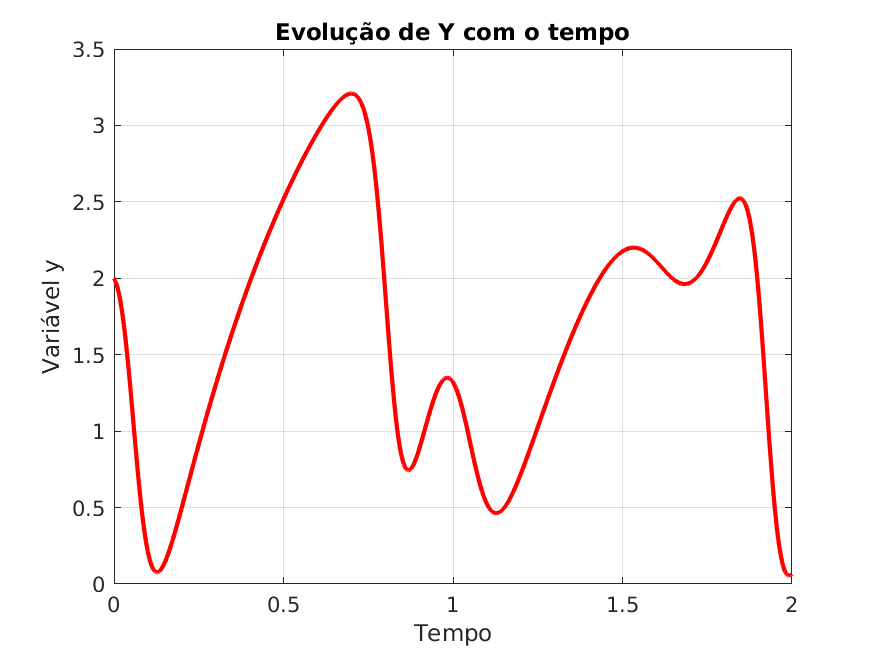
\includegraphics[scale = 0.55]{ploty_timescaled.png}\label{yts}}
        \caption{Comparação entre o sistema original e o escalonado para a variável Y}
    \end{figure}

    \begin{figure}[H]
        \subfloat[][Gráfico do sistema original]{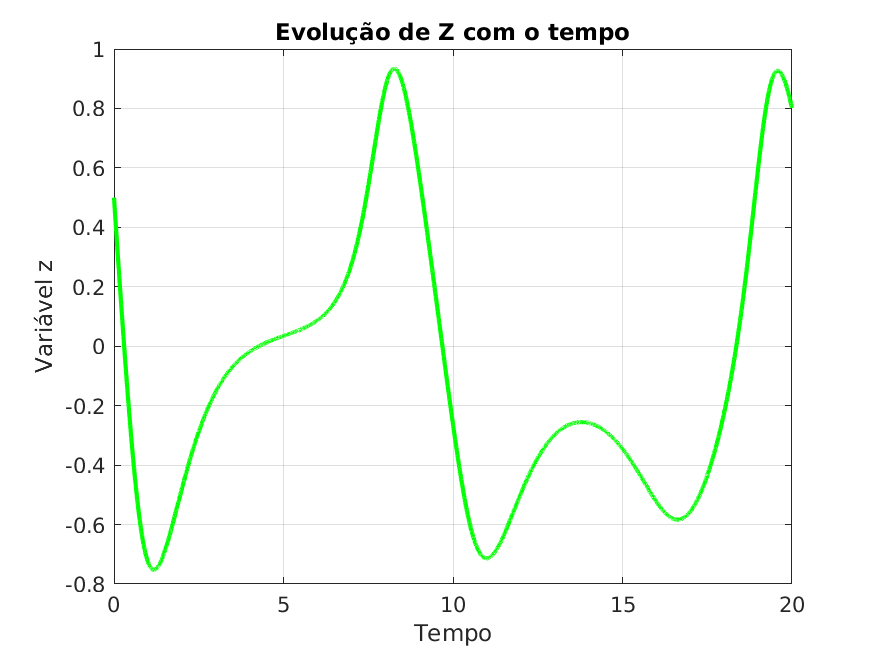
\includegraphics[scale = 0.55]{plotz.png}\label{zorig}}
        \subfloat[][Gráfico do sistema escalonado no tempo]{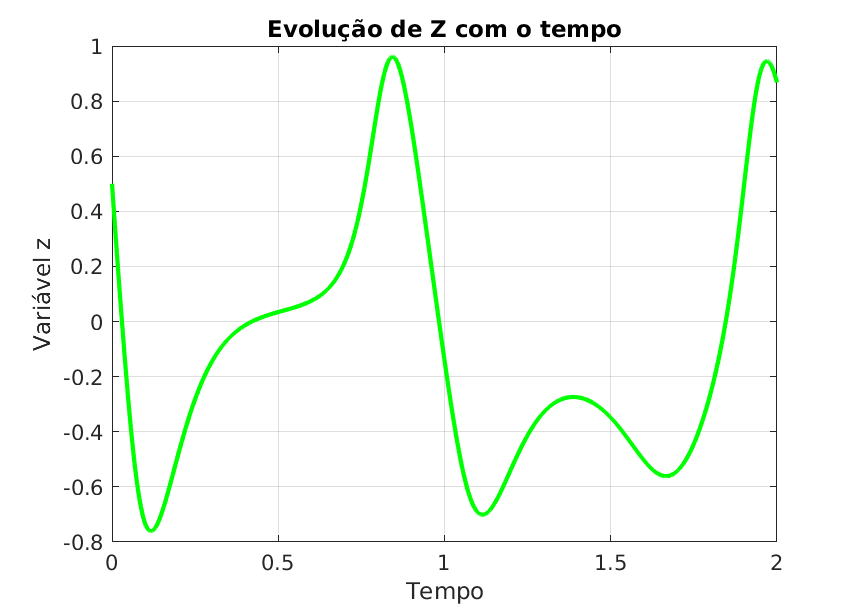
\includegraphics[scale = 0.55]{plotz_timescaled.png}\label{zts}}
        \caption{Comparação entre o sistema original e o escalonado para a variável Z}
    \end{figure}

    \begin{figure}[H]
        \subfloat[][Gráfico do sistema original]{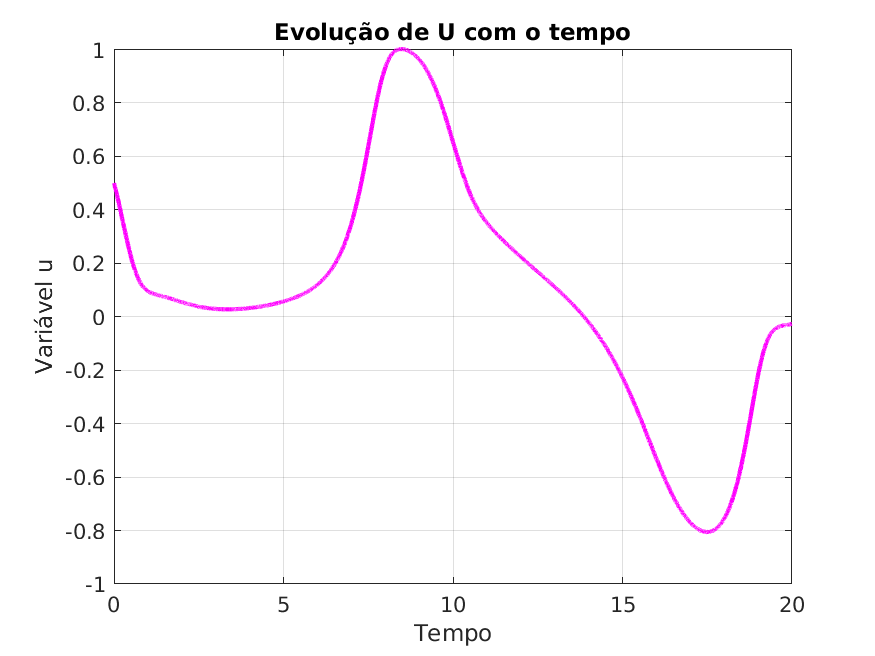
\includegraphics[scale = 0.55]{plotu.png}\label{uorig}}
        \subfloat[][Gráfico do sistema escalonado no tempo]{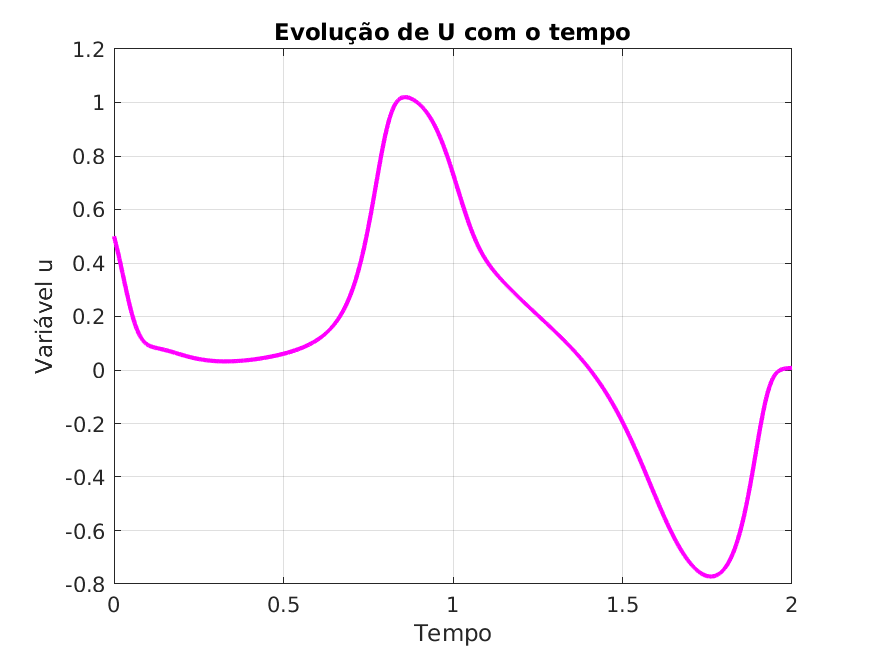
\includegraphics[scale = 0.55]{plotu_timescaled.png}\label{uts}}
        \caption{Comparação entre o sistema original e o escalonado para a variável U}
    \end{figure}


    \subsection{Escalonamento na amplitude}
    O escalonamento na amplitude do sistema pode ser feito com:
    \begin{enumerate}
        \item Divisão das condições iniciais pelo fator de escalonamento
        \item Multiplicação dos termos não lineares da equaçõ pelo fator de escalonamento
        \item Divisão dos termos constantes da equação pelo fator de escalonamento
    \end{enumerate}

    Nesse cas, o objetivo é que nenhuma variávelde estado assuma um valor absoluto maior que 1. Como podemos ver na figura \ref{origy}, o maior valor entre as variáveis de estado é 3,15, e por isso esse será o fator de escalonamento. Obteremos o sistema abaixo:
    
    \begin{equation}
        \left\{
            \begin{array}{l}
              \dot{x} = z + (y\times3.15 - a)x + u\\
              \dot{y} = \frac{1}{3.15} - by - x^2\times3.15\\
              \dot{z} = -x - cz\\
              \dot{u} = -dxy\times3.15 - ku
            \end{array}
          \right.
    \end{equation}
    Esse sistema está implementado no script \texttt{amplitude\_scaling.m}

    Nas figuras abaixo, podemos ver uma comparação entre os sinais originais e os escalonados na amplitude, que mostram que o escalonamento manteve a forma dos sistemas e diminuiu sua amplitude, conforme desejado.
    \begin{figure}[H]
        \subfloat[][Gráfico do sistema original]{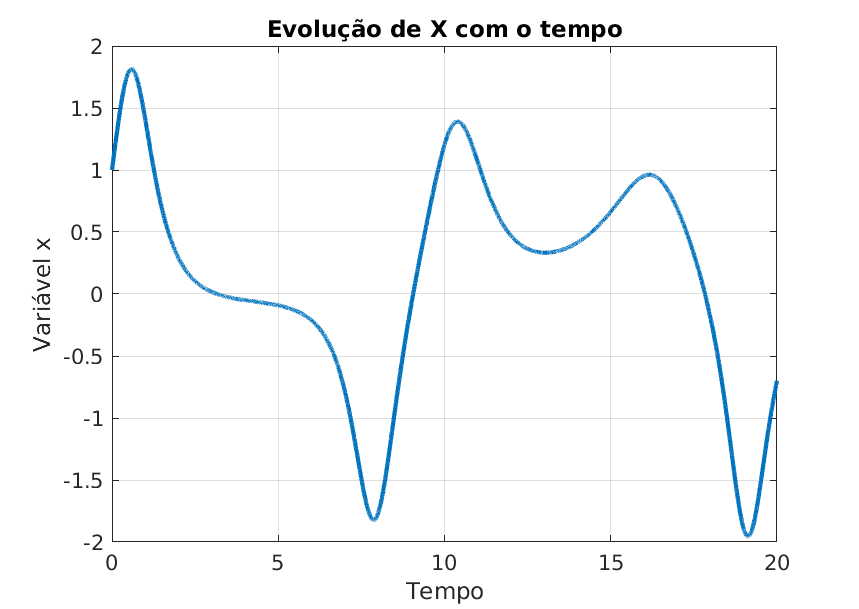
\includegraphics[scale = 0.55]{plotx.png}\label{xorigx}}
        \subfloat[][Gráfico do sistema escalonado na amplitude]{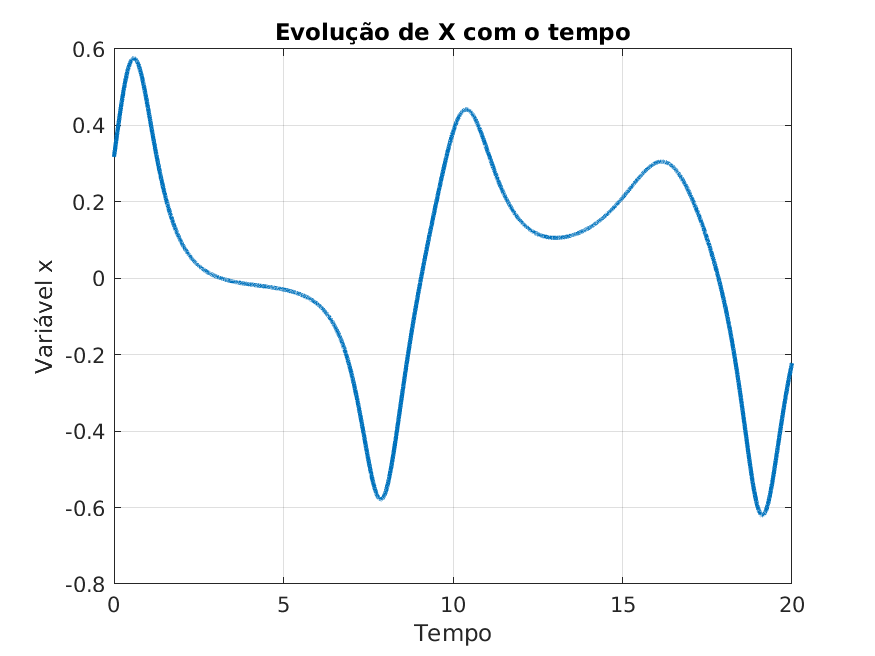
\includegraphics[scale = 0.55]{plotx_ampscaled.png}\label{xas}}
        \caption{Comparação entre o sistema original e o escalonado para a variável X}
    \end{figure}

    \begin{figure}[H]
        \subfloat[][Gráfico do sistema original]{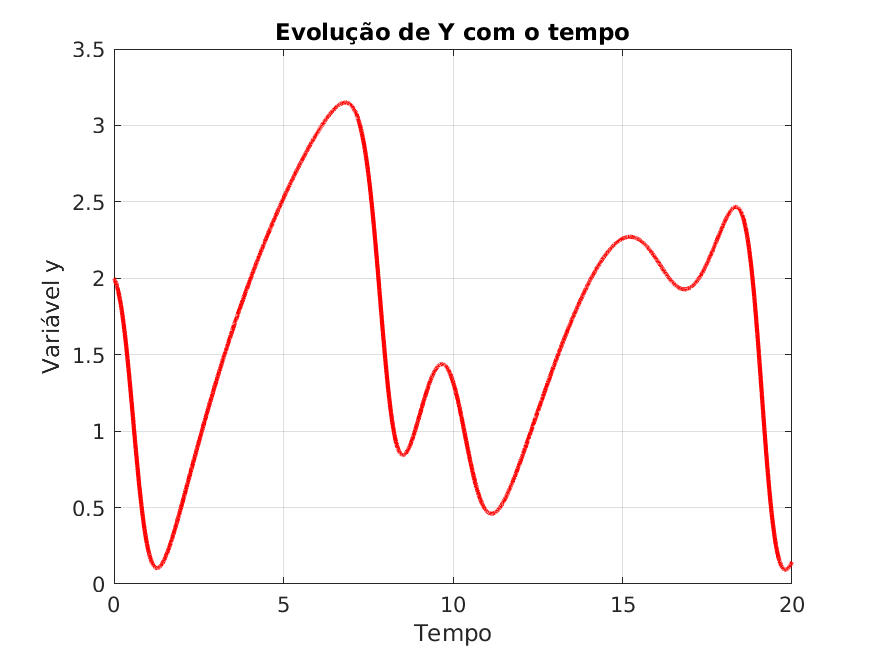
\includegraphics[scale = 0.55]{ploty.png}\label{yorigy}}
        \subfloat[][Gráfico do sistema escalonado na amplitude]{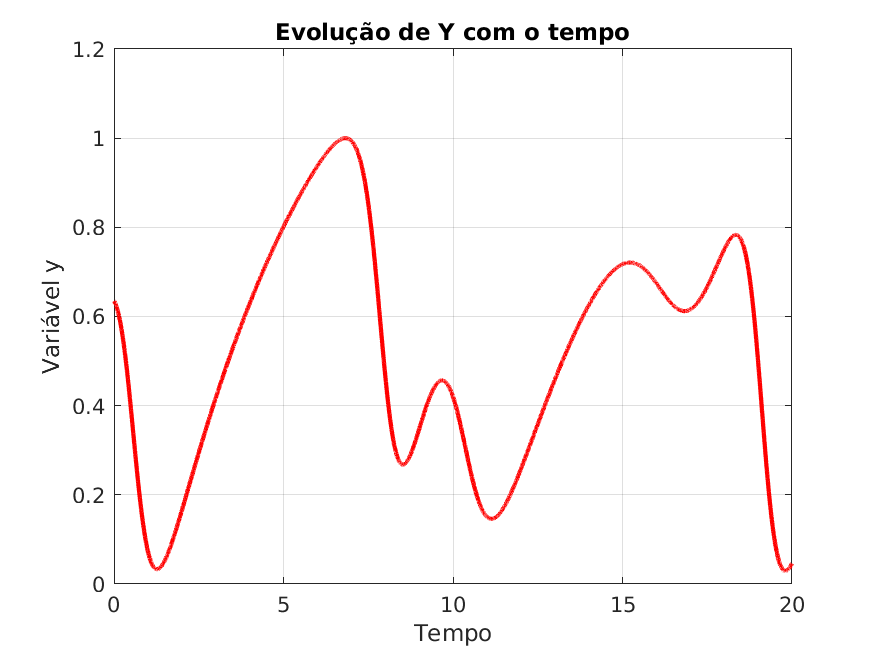
\includegraphics[scale = 0.55]{ploty_ampscaled.png}\label{yas}}
        \caption{Comparação entre o sistema original e o escalonado para a variável Y}
    \end{figure}

    \begin{figure}[H]
        \subfloat[][Gráfico do sistema original]{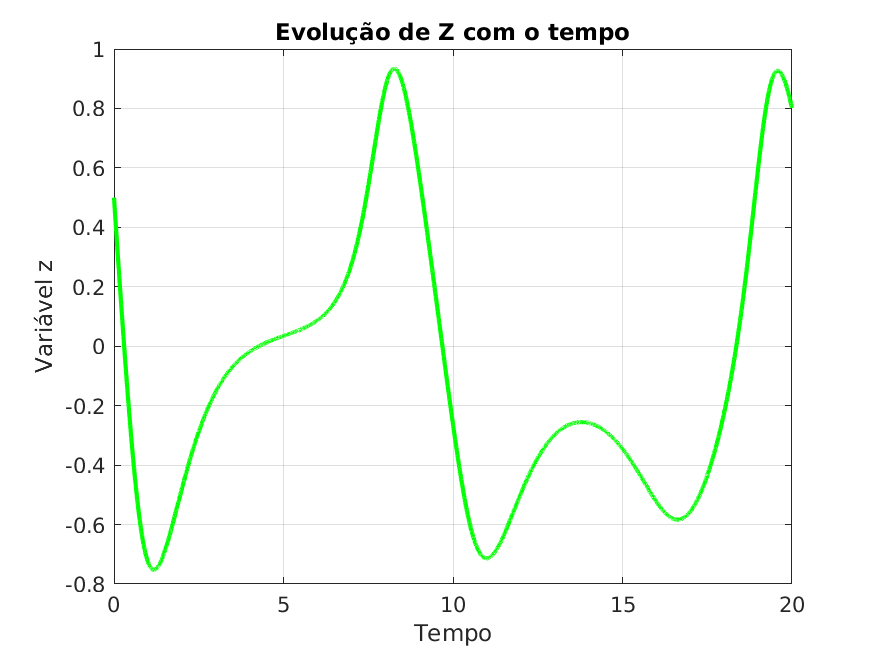
\includegraphics[scale = 0.55]{plotz.png}\label{zorigz}}
        \subfloat[][Gráfico do sistema escalonado na amplitude]{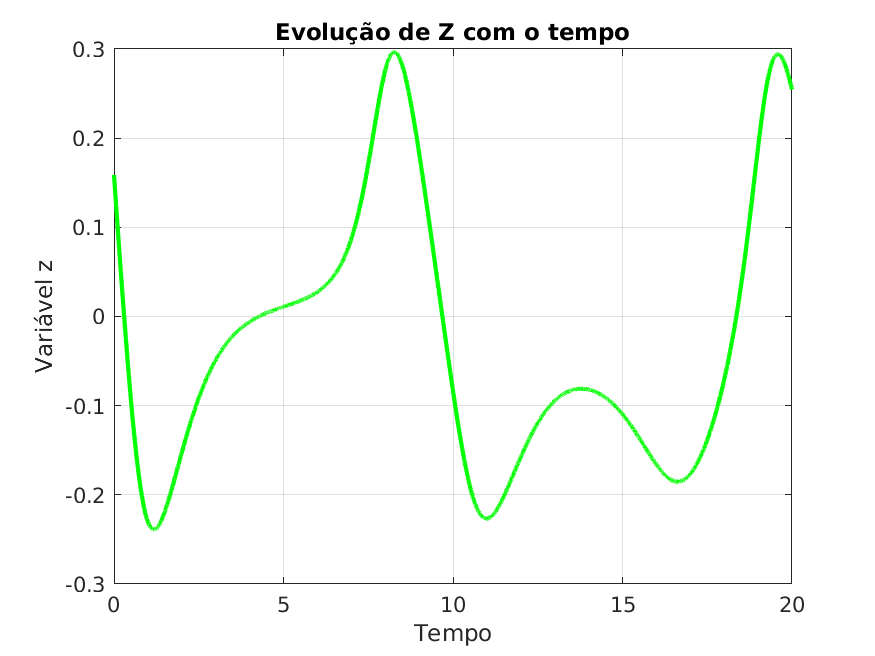
\includegraphics[scale = 0.55]{plotz_ampscaled.png}\label{zas}}
        \caption{Comparação entre o sistema original e o escalonado para a variável Z}
    \end{figure}

    \begin{figure}[H]
        \subfloat[][Gráfico do sistema original]{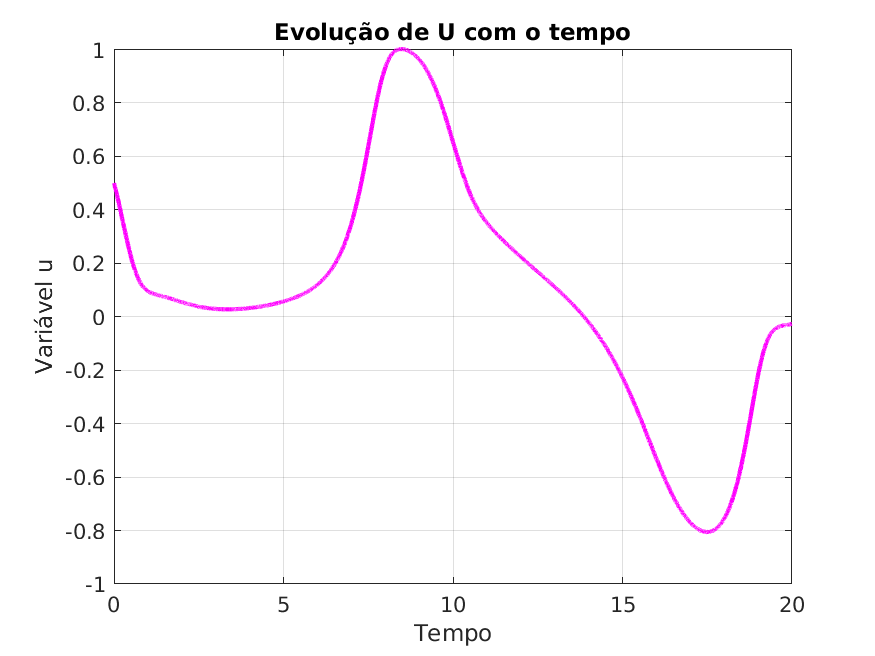
\includegraphics[scale = 0.55]{plotu.png}\label{uorigu}}
        \subfloat[][Gráfico do sistema escalonado na amplitude]{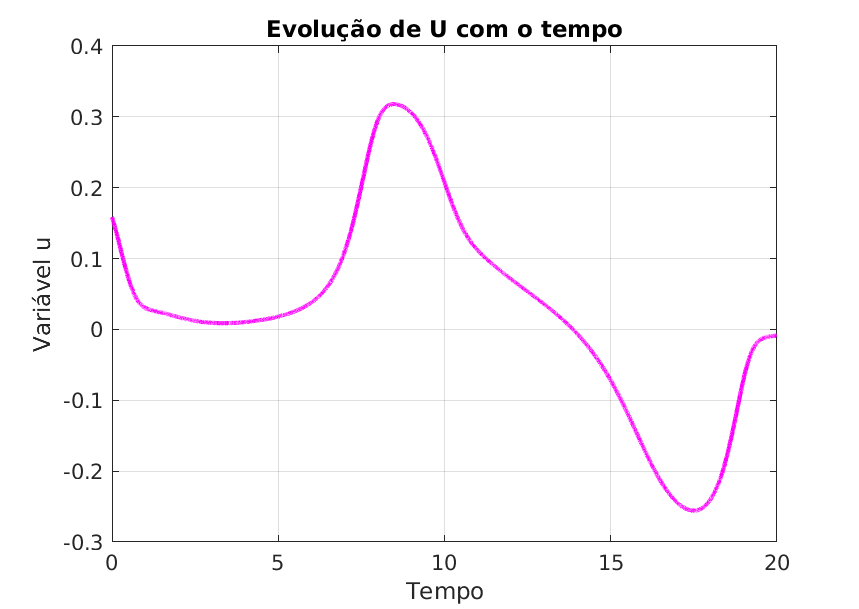
\includegraphics[scale = 0.55]{plotu_ampscaled.png}\label{uas}}
        \caption{Comparação entre o sistema original e o escalonado para a variável U}
    \end{figure}
    
\section{Diagramas de fase}
Foram feitos diagramas de fase para as equações do seguinte sistema:
\begin{equation}
    \left\{
        \begin{array}{l}
          \dot{x} = z + (y - a)x\\
          \dot{y} = 1 - by - x^2\\
          \dot{z} = -x - cz
        \end{array}
      \right.
\end{equation}
Foram escolhidas 10 condições iniciais igualmente espaçadas entre -4 e 4 para x, entre 0 e 4 para y e entre -2 e 2 para z. Os gráficos de fases duas a duas foram plotados no script \texttt{phase\_diagrams.m} e são mostrados abaixo:
\begin{figure}[H]
    \subfloat[][Gráfico das variáveis X e Y]{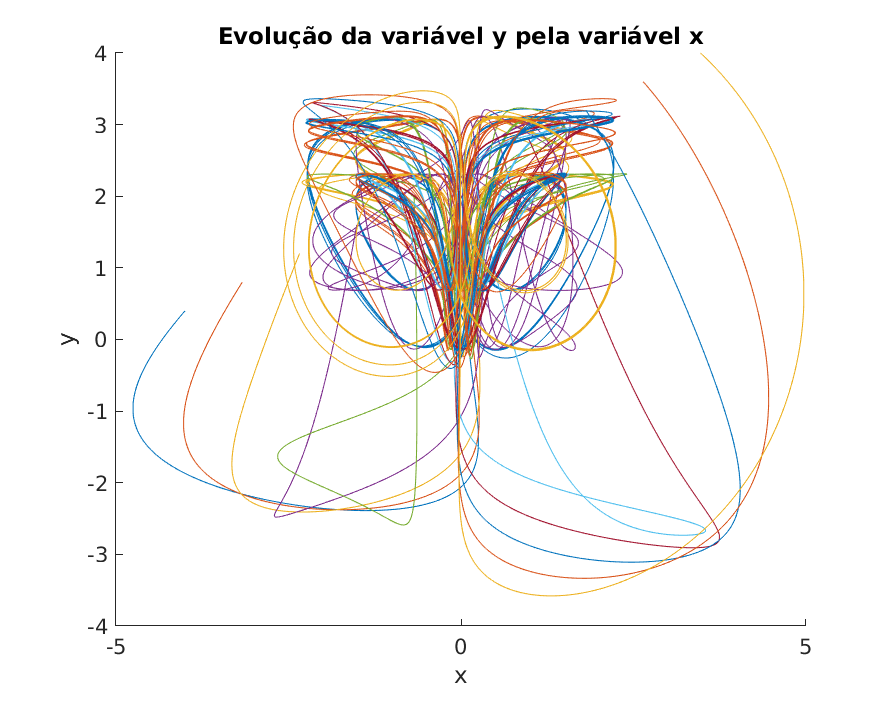
\includegraphics[scale = 0.5]{xy.png}\label{xy}}
    \subfloat[][Gráfico das variáveis Y e Z]{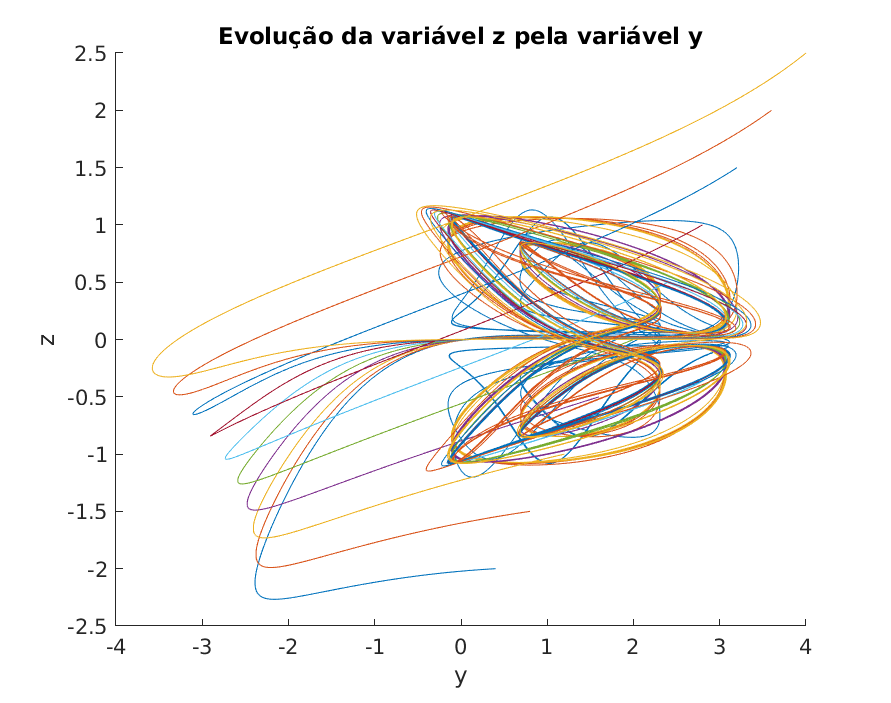
\includegraphics[scale = 0.5]{yz.png}\label{yz}} \par
    \subfloat[][Gráfico das variáveis X e Z]{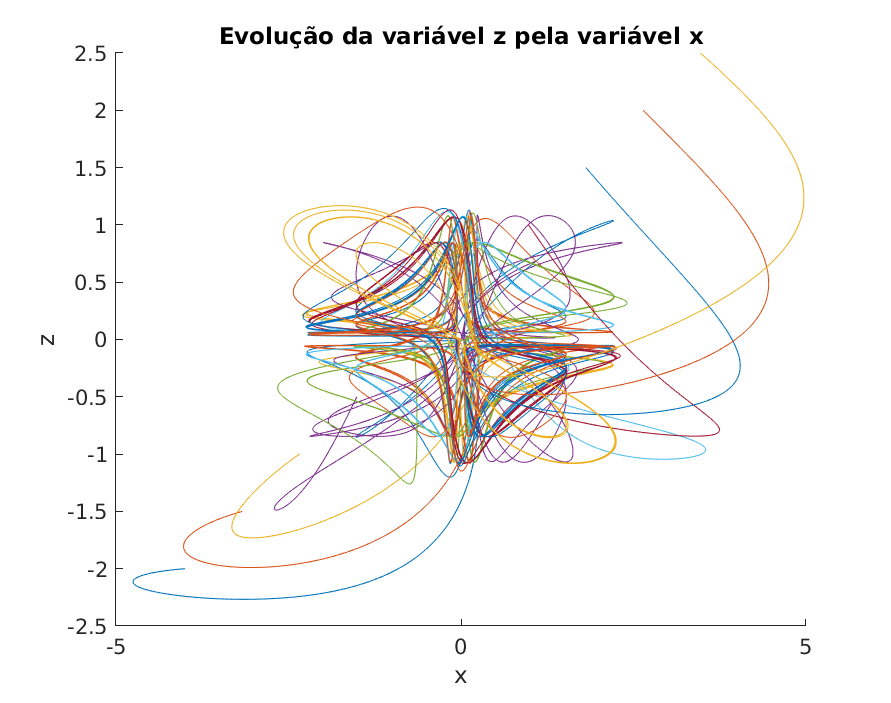
\includegraphics[scale = 0.5]{xz.png}\label{xz}}
    \subfloat[][Gráfico das três variáveis]{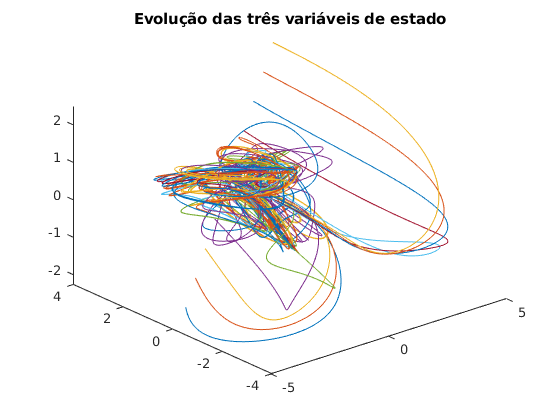
\includegraphics[scale = 0.5]{xyz.png}\label{xyz}}
    \caption{Diagramas das variáveis do sistema}
\end{figure}
\end{document}